% Created by tikzDevice version 0.9 on 2015-12-20 19:34:29
% !TEX encoding = UTF-8 Unicode

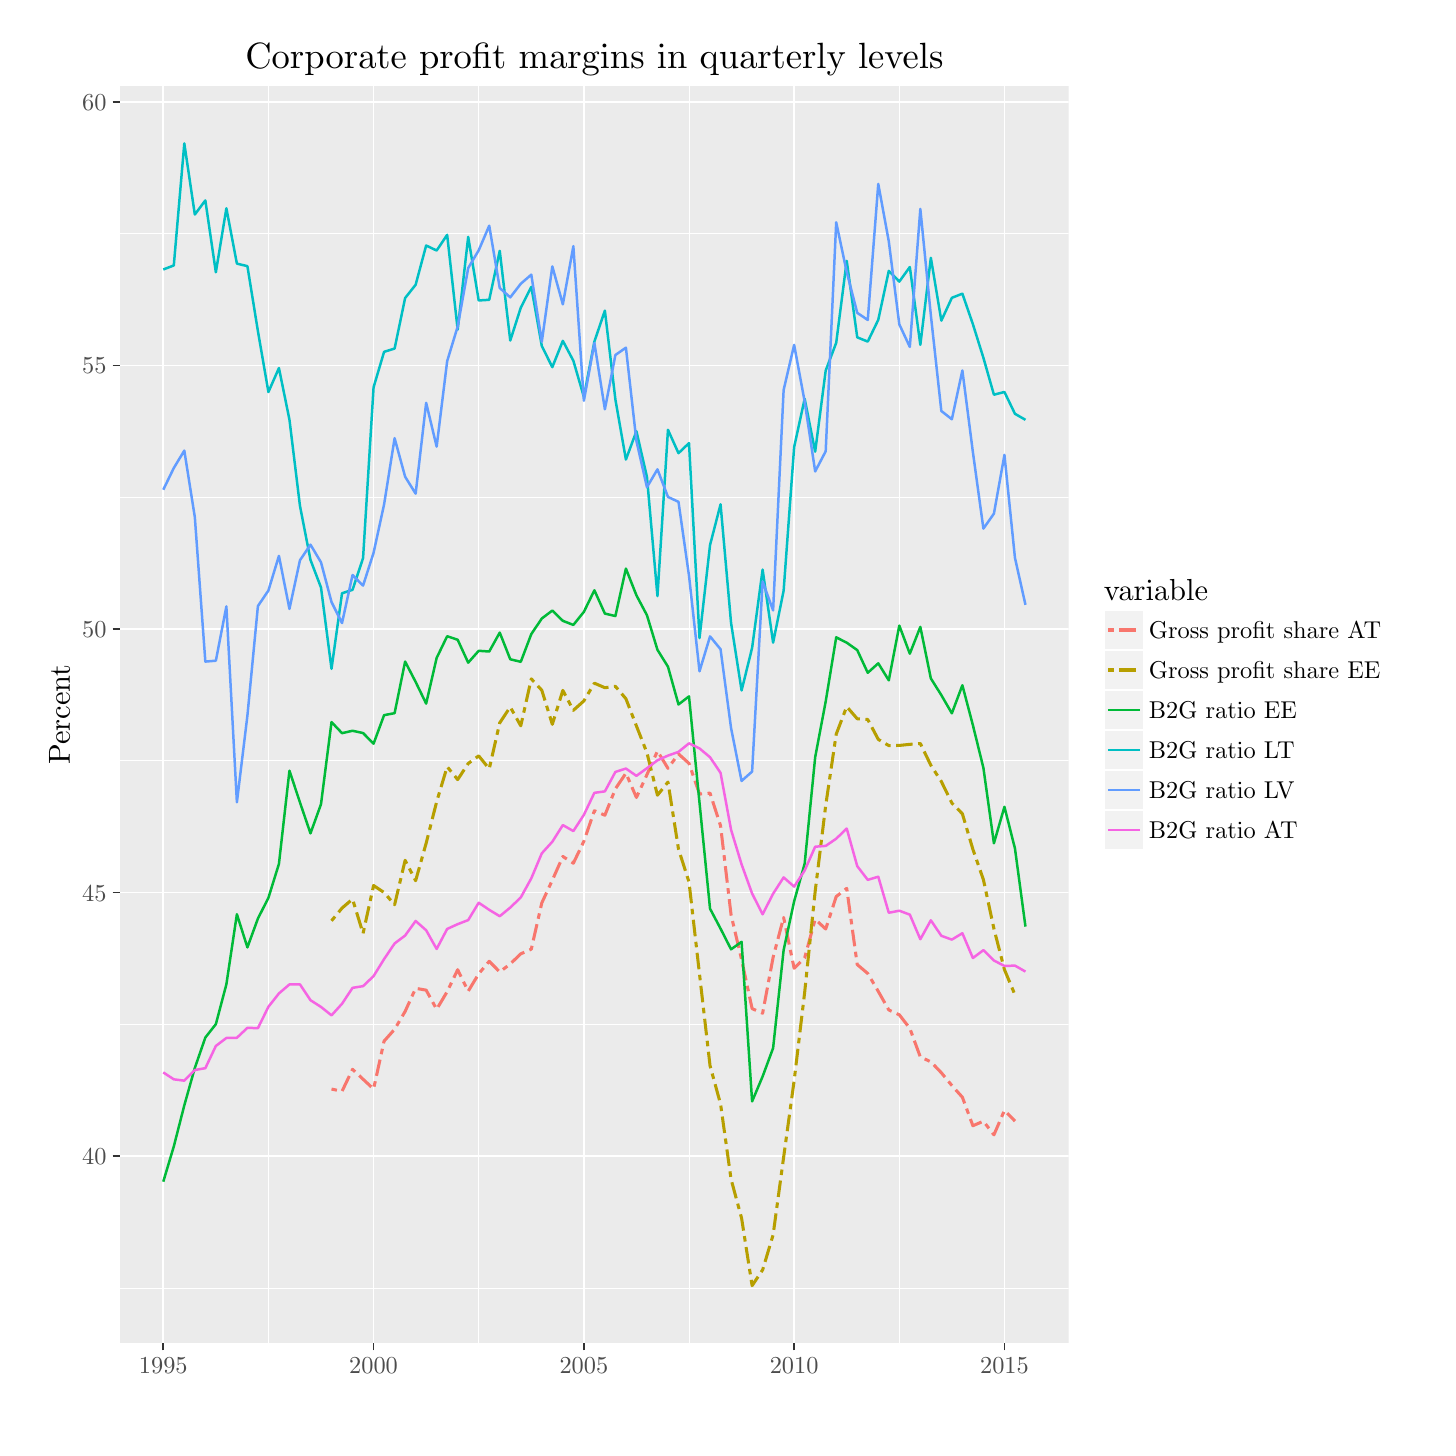
\begin{tikzpicture}[x=1pt,y=1pt]
\definecolor{fillColor}{RGB}{255,255,255}
\path[use as bounding box,fill=fillColor,fill opacity=0.00] (0,0) rectangle (505.89,505.89);
\begin{scope}
\path[clip] (  0.00,  0.00) rectangle (505.89,505.89);
\definecolor{drawColor}{RGB}{255,255,255}
\definecolor{fillColor}{RGB}{255,255,255}

\path[draw=drawColor,line width= 0.6pt,line join=round,line cap=round,fill=fillColor] (  0.00,  0.00) rectangle (505.89,505.89);
\end{scope}
\begin{scope}
\path[clip] ( 33.42, 30.69) rectangle (376.13,484.70);
\definecolor{fillColor}{gray}{0.92}

\path[fill=fillColor] ( 33.42, 30.69) rectangle (376.13,484.70);
\definecolor{drawColor}{RGB}{255,255,255}

\path[draw=drawColor,line width= 0.3pt,line join=round] ( 33.42, 50.46) --
	(376.13, 50.46);

\path[draw=drawColor,line width= 0.3pt,line join=round] ( 33.42,145.71) --
	(376.13,145.71);

\path[draw=drawColor,line width= 0.3pt,line join=round] ( 33.42,240.96) --
	(376.13,240.96);

\path[draw=drawColor,line width= 0.3pt,line join=round] ( 33.42,336.21) --
	(376.13,336.21);

\path[draw=drawColor,line width= 0.3pt,line join=round] ( 33.42,431.46) --
	(376.13,431.46);

\path[draw=drawColor,line width= 0.3pt,line join=round] ( 86.99, 30.69) --
	( 86.99,484.70);

\path[draw=drawColor,line width= 0.3pt,line join=round] (162.98, 30.69) --
	(162.98,484.70);

\path[draw=drawColor,line width= 0.3pt,line join=round] (238.97, 30.69) --
	(238.97,484.70);

\path[draw=drawColor,line width= 0.3pt,line join=round] (314.96, 30.69) --
	(314.96,484.70);

\path[draw=drawColor,line width= 0.6pt,line join=round] ( 33.42, 98.08) --
	(376.13, 98.08);

\path[draw=drawColor,line width= 0.6pt,line join=round] ( 33.42,193.33) --
	(376.13,193.33);

\path[draw=drawColor,line width= 0.6pt,line join=round] ( 33.42,288.58) --
	(376.13,288.58);

\path[draw=drawColor,line width= 0.6pt,line join=round] ( 33.42,383.83) --
	(376.13,383.83);

\path[draw=drawColor,line width= 0.6pt,line join=round] ( 33.42,479.08) --
	(376.13,479.08);

\path[draw=drawColor,line width= 0.6pt,line join=round] ( 49.00, 30.69) --
	( 49.00,484.70);

\path[draw=drawColor,line width= 0.6pt,line join=round] (124.99, 30.69) --
	(124.99,484.70);

\path[draw=drawColor,line width= 0.6pt,line join=round] (200.98, 30.69) --
	(200.98,484.70);

\path[draw=drawColor,line width= 0.6pt,line join=round] (276.96, 30.69) --
	(276.96,484.70);

\path[draw=drawColor,line width= 0.6pt,line join=round] (352.95, 30.69) --
	(352.95,484.70);
\definecolor{drawColor}{RGB}{248,118,109}

\path[draw=drawColor,line width= 1.1pt,dash pattern=on 2pt off 2pt on 6pt off 2pt ,line join=round] (109.79,122.36) --
	(113.59,121.55) --
	(117.39,129.50) --
	(121.19,125.91) --
	(124.99,122.37) --
	(128.79,139.69) --
	(132.59,143.95) --
	(136.39,150.41) --
	(140.19,158.76) --
	(143.99,158.10) --
	(147.78,151.17) --
	(151.58,157.56) --
	(155.38,165.48) --
	(159.18,157.69) --
	(162.98,164.01) --
	(166.78,168.52) --
	(170.58,164.68) --
	(174.38,167.56) --
	(178.18,171.22) --
	(181.98,172.91) --
	(185.78,189.63) --
	(189.58,197.82) --
	(193.38,206.40) --
	(197.18,203.97) --
	(200.98,211.89) --
	(204.78,222.94) --
	(208.57,221.30) --
	(212.37,230.83) --
	(216.17,236.50) --
	(219.97,227.71) --
	(223.77,235.96) --
	(227.57,244.49) --
	(231.37,238.25) --
	(235.17,243.47) --
	(238.97,240.03) --
	(242.77,228.96) --
	(246.57,229.29) --
	(250.37,217.52) --
	(254.17,185.29) --
	(257.97,169.16) --
	(261.77,151.42) --
	(265.57,149.77) --
	(269.36,169.95) --
	(273.16,184.36) --
	(276.96,166.00) --
	(280.76,169.76) --
	(284.56,183.71) --
	(288.36,180.19) --
	(292.16,191.90) --
	(295.96,194.87) --
	(299.76,167.33) --
	(303.56,164.12) --
	(307.36,157.66) --
	(311.16,150.94) --
	(314.96,149.19) --
	(318.76,144.31) --
	(322.56,133.94) --
	(326.36,132.21) --
	(330.15,128.25) --
	(333.95,123.64) --
	(337.75,119.41) --
	(341.55,109.10) --
	(345.35,110.74) --
	(349.15,105.81) --
	(352.95,114.64) --
	(356.75,110.79);
\definecolor{drawColor}{RGB}{183,159,0}

\path[draw=drawColor,line width= 1.1pt,dash pattern=on 2pt off 2pt on 6pt off 2pt ,line join=round] (109.79,183.15) --
	(113.59,187.75) --
	(117.39,191.01) --
	(121.19,178.58) --
	(124.99,195.91) --
	(128.79,193.39) --
	(132.59,188.95) --
	(136.39,205.03) --
	(140.19,197.65) --
	(143.99,211.20) --
	(147.78,226.16) --
	(151.58,238.83) --
	(155.38,234.18) --
	(159.18,239.99) --
	(162.98,242.76) --
	(166.78,238.05) --
	(170.58,254.71) --
	(174.38,260.42) --
	(178.18,253.61) --
	(181.98,270.59) --
	(185.78,266.46) --
	(189.58,254.15) --
	(193.38,266.42) --
	(197.18,259.21) --
	(200.98,262.61) --
	(204.78,269.02) --
	(208.57,267.38) --
	(212.37,267.88) --
	(216.17,263.40) --
	(219.97,253.56) --
	(223.77,243.88) --
	(227.57,228.53) --
	(231.37,233.29) --
	(235.17,209.07) --
	(238.97,197.18) --
	(242.77,163.84) --
	(246.57,130.79) --
	(250.37,116.94) --
	(254.17, 89.78) --
	(257.97, 75.69) --
	(261.77, 51.32) --
	(265.57, 57.00) --
	(269.36, 69.67) --
	(273.16, 97.70) --
	(276.96,125.40) --
	(280.76,157.27) --
	(284.56,193.79) --
	(288.36,224.79) --
	(292.16,250.58) --
	(295.96,260.56) --
	(299.76,256.15) --
	(303.56,255.89) --
	(307.36,248.72) --
	(311.16,246.47) --
	(314.96,246.52) --
	(318.76,246.92) --
	(322.56,247.22) --
	(326.36,239.35) --
	(330.15,233.49) --
	(333.95,225.72) --
	(337.75,221.83) --
	(341.55,208.99) --
	(345.35,198.02) --
	(349.15,180.29) --
	(352.95,165.53) --
	(356.75,156.42);
\definecolor{drawColor}{RGB}{0,186,56}

\path[draw=drawColor,line width= 0.9pt,line join=round] ( 49.00, 88.89) --
	( 52.80,101.62) --
	( 56.60,116.47) --
	( 60.40,129.99) --
	( 64.20,140.97) --
	( 68.00,145.81) --
	( 71.80,160.19) --
	( 75.60,185.53) --
	( 79.40,173.56) --
	( 83.20,183.97) --
	( 86.99,191.46) --
	( 90.79,203.71) --
	( 94.59,237.40) --
	( 98.39,225.93) --
	(102.19,214.75) --
	(105.99,225.29) --
	(109.79,254.97) --
	(113.59,250.96) --
	(117.39,251.82) --
	(121.19,251.00) --
	(124.99,247.17) --
	(128.79,257.47) --
	(132.59,258.18) --
	(136.39,276.83) --
	(140.19,269.47) --
	(143.99,261.64) --
	(147.78,278.14) --
	(151.58,285.99) --
	(155.38,284.71) --
	(159.18,276.43) --
	(162.98,280.72) --
	(166.78,280.46) --
	(170.58,287.30) --
	(174.38,277.66) --
	(178.18,276.74) --
	(181.98,286.75) --
	(185.78,292.40) --
	(189.58,295.26) --
	(193.38,291.55) --
	(197.18,290.07) --
	(200.98,294.79) --
	(204.78,302.59) --
	(208.57,294.17) --
	(212.37,293.28) --
	(216.17,310.42) --
	(219.97,300.77) --
	(223.77,293.59) --
	(227.57,281.07) --
	(231.37,274.98) --
	(235.17,261.33) --
	(238.97,264.25) --
	(242.77,225.77) --
	(246.57,187.53) --
	(250.37,180.32) --
	(254.17,172.85) --
	(257.97,175.56) --
	(261.77,117.90) --
	(265.57,126.91) --
	(269.36,137.17) --
	(273.16,172.56) --
	(276.96,190.22) --
	(280.76,203.77) --
	(284.56,242.26) --
	(288.36,262.38) --
	(292.16,285.58) --
	(295.96,283.66) --
	(299.76,280.97) --
	(303.56,272.78) --
	(307.36,276.20) --
	(311.16,270.06) --
	(314.96,289.83) --
	(318.76,279.68) --
	(322.56,289.35) --
	(326.36,270.74) --
	(330.15,264.70) --
	(333.95,258.13) --
	(337.75,268.27) --
	(341.55,253.85) --
	(345.35,238.42) --
	(349.15,211.16) --
	(352.95,224.35) --
	(356.75,209.31) --
	(360.55,181.06);
\definecolor{drawColor}{RGB}{0,191,196}

\path[draw=drawColor,line width= 0.9pt,line join=round] ( 49.00,418.50) --
	( 52.80,419.97) --
	( 56.60,464.06) --
	( 60.40,438.37) --
	( 64.20,443.46) --
	( 68.00,417.49) --
	( 71.80,440.63) --
	( 75.60,420.62) --
	( 79.40,419.71) --
	( 83.20,396.21) --
	( 86.99,374.23) --
	( 90.79,382.89) --
	( 94.59,364.25) --
	( 98.39,333.10) --
	(102.19,313.58) --
	(105.99,303.59) --
	(109.79,274.22) --
	(113.59,301.51) --
	(117.39,302.75) --
	(121.19,314.21) --
	(124.99,375.94) --
	(128.79,388.76) --
	(132.59,389.93) --
	(136.39,408.19) --
	(140.19,412.99) --
	(143.99,427.17) --
	(147.78,425.36) --
	(151.58,431.02) --
	(155.38,396.74) --
	(159.18,430.29) --
	(162.98,407.31) --
	(166.78,407.55) --
	(170.58,425.25) --
	(174.38,392.82) --
	(178.18,404.69) --
	(181.98,412.22) --
	(185.78,390.85) --
	(189.58,383.21) --
	(193.38,392.72) --
	(197.18,385.54) --
	(200.98,372.46) --
	(204.78,392.46) --
	(208.57,403.65) --
	(212.37,371.53) --
	(216.17,349.83) --
	(219.97,360.07) --
	(223.77,343.58) --
	(227.57,300.50) --
	(231.37,360.57) --
	(235.17,352.13) --
	(238.97,355.76) --
	(242.77,285.33) --
	(246.57,318.93) --
	(250.37,333.66) --
	(254.17,290.76) --
	(257.97,266.38) --
	(261.77,281.77) --
	(265.57,310.08) --
	(269.36,283.67) --
	(273.16,302.42) --
	(276.96,354.32) --
	(280.76,371.78) --
	(284.56,352.67) --
	(288.36,381.97) --
	(292.16,392.00) --
	(295.96,421.63) --
	(299.76,393.99) --
	(303.56,392.45) --
	(307.36,400.32) --
	(311.16,417.99) --
	(314.96,414.14) --
	(318.76,419.39) --
	(322.56,391.28) --
	(326.36,422.74) --
	(330.15,400.02) --
	(333.95,408.26) --
	(337.75,409.77) --
	(341.55,398.75) --
	(345.35,386.59) --
	(349.15,373.26) --
	(352.95,374.25) --
	(356.75,366.36) --
	(360.55,364.18);
\definecolor{drawColor}{RGB}{97,156,255}

\path[draw=drawColor,line width= 0.9pt,line join=round] ( 49.00,338.92) --
	( 52.80,346.76) --
	( 56.60,353.06) --
	( 60.40,329.03) --
	( 64.20,276.82) --
	( 68.00,277.14) --
	( 71.80,296.76) --
	( 75.60,225.97) --
	( 79.40,257.30) --
	( 83.20,296.89) --
	( 86.99,302.50) --
	( 90.79,315.03) --
	( 94.59,295.85) --
	( 98.39,313.43) --
	(102.19,319.06) --
	(105.99,312.71) --
	(109.79,298.34) --
	(113.59,290.75) --
	(117.39,308.10) --
	(121.19,304.28) --
	(124.99,316.13) --
	(128.79,333.62) --
	(132.59,357.54) --
	(136.39,343.63) --
	(140.19,337.50) --
	(143.99,370.33) --
	(147.78,354.50) --
	(151.58,385.37) --
	(155.38,397.89) --
	(159.18,419.02) --
	(162.98,425.43) --
	(166.78,434.33) --
	(170.58,411.82) --
	(174.38,408.43) --
	(178.18,413.35) --
	(181.98,416.64) --
	(185.78,392.38) --
	(189.58,419.62) --
	(193.38,405.91) --
	(197.18,426.93) --
	(200.98,371.07) --
	(204.78,391.95) --
	(208.57,367.99) --
	(212.37,387.60) --
	(216.17,390.25) --
	(219.97,356.54) --
	(223.77,339.84) --
	(227.57,346.29) --
	(231.37,336.31) --
	(235.17,334.55) --
	(238.97,307.85) --
	(242.77,273.32) --
	(246.57,285.92) --
	(250.37,281.28) --
	(254.17,252.78) --
	(257.97,233.69) --
	(261.77,237.08) --
	(265.57,305.74) --
	(269.36,295.31) --
	(273.16,374.95) --
	(276.96,391.26) --
	(280.76,370.81) --
	(284.56,345.54) --
	(288.36,352.81) --
	(292.16,435.56) --
	(295.96,417.60) --
	(299.76,402.84) --
	(303.56,400.27) --
	(307.36,449.42) --
	(311.16,428.67) --
	(314.96,398.69) --
	(318.76,390.52) --
	(322.56,440.39) --
	(326.36,401.98) --
	(330.15,367.37) --
	(333.95,364.39) --
	(337.75,382.02) --
	(341.55,352.52) --
	(345.35,324.87) --
	(349.15,330.29) --
	(352.95,351.51) --
	(356.75,314.32) --
	(360.55,297.33);
\definecolor{drawColor}{RGB}{245,100,227}

\path[draw=drawColor,line width= 0.9pt,line join=round] ( 49.00,128.38) --
	( 52.80,125.87) --
	( 56.60,125.39) --
	( 60.40,129.24) --
	( 64.20,129.90) --
	( 68.00,137.93) --
	( 71.80,140.82) --
	( 75.60,140.89) --
	( 79.40,144.48) --
	( 83.20,144.36) --
	( 86.99,152.08) --
	( 90.79,156.91) --
	( 94.59,160.17) --
	( 98.39,160.17) --
	(102.19,154.47) --
	(105.99,152.03) --
	(109.79,148.99) --
	(113.59,153.18) --
	(117.39,158.93) --
	(121.19,159.54) --
	(124.99,163.17) --
	(128.79,169.32) --
	(132.59,174.96) --
	(136.39,177.83) --
	(140.19,183.09) --
	(143.99,179.73) --
	(147.78,172.98) --
	(151.58,180.21) --
	(155.38,181.94) --
	(159.18,183.41) --
	(162.98,189.68) --
	(166.78,187.12) --
	(170.58,184.81) --
	(174.38,187.94) --
	(178.18,191.59) --
	(181.98,198.49) --
	(185.78,207.54) --
	(189.58,211.73) --
	(193.38,217.74) --
	(197.18,215.58) --
	(200.98,221.44) --
	(204.78,229.40) --
	(208.57,229.92) --
	(212.37,236.95) --
	(216.17,238.17) --
	(219.97,235.54) --
	(223.77,238.28) --
	(227.57,241.15) --
	(231.37,242.85) --
	(235.17,244.19) --
	(238.97,247.29) --
	(242.77,245.44) --
	(246.57,242.26) --
	(250.37,236.61) --
	(254.17,216.04) --
	(257.97,203.54) --
	(261.77,193.02) --
	(265.57,185.52) --
	(269.36,192.94) --
	(273.16,198.84) --
	(276.96,195.51) --
	(280.76,201.34) --
	(284.56,209.93) --
	(288.36,210.22) --
	(292.16,212.82) --
	(295.96,216.50) --
	(299.76,202.91) --
	(303.56,197.95) --
	(307.36,199.09) --
	(311.16,186.06) --
	(314.96,186.80) --
	(318.76,185.38) --
	(322.56,176.49) --
	(326.36,183.34) --
	(330.15,177.73) --
	(333.95,176.36) --
	(337.75,178.67) --
	(341.55,169.70) --
	(345.35,172.55) --
	(349.15,168.81) --
	(352.95,166.84) --
	(356.75,166.96) --
	(360.55,164.80);
\end{scope}
\begin{scope}
\path[clip] (  0.00,  0.00) rectangle (505.89,505.89);
\definecolor{drawColor}{gray}{0.30}

\node[text=drawColor,anchor=base east,inner sep=0pt, outer sep=0pt, scale=  0.88] at ( 28.47, 95.05) {40};

\node[text=drawColor,anchor=base east,inner sep=0pt, outer sep=0pt, scale=  0.88] at ( 28.47,190.30) {45};

\node[text=drawColor,anchor=base east,inner sep=0pt, outer sep=0pt, scale=  0.88] at ( 28.47,285.55) {50};

\node[text=drawColor,anchor=base east,inner sep=0pt, outer sep=0pt, scale=  0.88] at ( 28.47,380.80) {55};

\node[text=drawColor,anchor=base east,inner sep=0pt, outer sep=0pt, scale=  0.88] at ( 28.47,476.05) {60};
\end{scope}
\begin{scope}
\path[clip] (  0.00,  0.00) rectangle (505.89,505.89);
\definecolor{drawColor}{gray}{0.20}

\path[draw=drawColor,line width= 0.6pt,line join=round] ( 30.67, 98.08) --
	( 33.42, 98.08);

\path[draw=drawColor,line width= 0.6pt,line join=round] ( 30.67,193.33) --
	( 33.42,193.33);

\path[draw=drawColor,line width= 0.6pt,line join=round] ( 30.67,288.58) --
	( 33.42,288.58);

\path[draw=drawColor,line width= 0.6pt,line join=round] ( 30.67,383.83) --
	( 33.42,383.83);

\path[draw=drawColor,line width= 0.6pt,line join=round] ( 30.67,479.08) --
	( 33.42,479.08);
\end{scope}
\begin{scope}
\path[clip] (  0.00,  0.00) rectangle (505.89,505.89);
\definecolor{drawColor}{gray}{0.20}

\path[draw=drawColor,line width= 0.6pt,line join=round] ( 49.00, 27.94) --
	( 49.00, 30.69);

\path[draw=drawColor,line width= 0.6pt,line join=round] (124.99, 27.94) --
	(124.99, 30.69);

\path[draw=drawColor,line width= 0.6pt,line join=round] (200.98, 27.94) --
	(200.98, 30.69);

\path[draw=drawColor,line width= 0.6pt,line join=round] (276.96, 27.94) --
	(276.96, 30.69);

\path[draw=drawColor,line width= 0.6pt,line join=round] (352.95, 27.94) --
	(352.95, 30.69);
\end{scope}
\begin{scope}
\path[clip] (  0.00,  0.00) rectangle (505.89,505.89);
\definecolor{drawColor}{gray}{0.30}

\node[text=drawColor,anchor=base,inner sep=0pt, outer sep=0pt, scale=  0.88] at ( 49.00, 19.68) {1995};

\node[text=drawColor,anchor=base,inner sep=0pt, outer sep=0pt, scale=  0.88] at (124.99, 19.68) {2000};

\node[text=drawColor,anchor=base,inner sep=0pt, outer sep=0pt, scale=  0.88] at (200.98, 19.68) {2005};

\node[text=drawColor,anchor=base,inner sep=0pt, outer sep=0pt, scale=  0.88] at (276.96, 19.68) {2010};

\node[text=drawColor,anchor=base,inner sep=0pt, outer sep=0pt, scale=  0.88] at (352.95, 19.68) {2015};
\end{scope}
\begin{scope}
\path[clip] (  0.00,  0.00) rectangle (505.89,505.89);
\definecolor{drawColor}{RGB}{0,0,0}

\node[text=drawColor,anchor=base,inner sep=0pt, outer sep=0pt, scale=  1.10] at (204.78,  7.70) {};
\end{scope}
\begin{scope}
\path[clip] (  0.00,  0.00) rectangle (505.89,505.89);
\definecolor{drawColor}{RGB}{0,0,0}

\node[text=drawColor,rotate= 90.00,anchor=base,inner sep=0pt, outer sep=0pt, scale=  1.10] at ( 15.28,257.69) {Percent};
\end{scope}
\begin{scope}
\path[clip] (  0.00,  0.00) rectangle (505.89,505.89);
\definecolor{fillColor}{RGB}{255,255,255}

\path[fill=fillColor] (384.66,204.47) rectangle (491.85,310.92);
\end{scope}
\begin{scope}
\path[clip] (  0.00,  0.00) rectangle (505.89,505.89);
\definecolor{drawColor}{RGB}{0,0,0}

\node[text=drawColor,anchor=base west,inner sep=0pt, outer sep=0pt, scale=  1.10] at (388.93,299.07) {variable};
\end{scope}
\begin{scope}
\path[clip] (  0.00,  0.00) rectangle (505.89,505.89);
\definecolor{drawColor}{RGB}{255,255,255}
\definecolor{fillColor}{gray}{0.95}

\path[draw=drawColor,line width= 0.6pt,line join=round,line cap=round,fill=fillColor] (388.93,281.01) rectangle (403.38,295.46);
\end{scope}
\begin{scope}
\path[clip] (  0.00,  0.00) rectangle (505.89,505.89);
\definecolor{drawColor}{RGB}{248,118,109}

\path[draw=drawColor,line width= 1.1pt,dash pattern=on 2pt off 2pt on 6pt off 2pt ,line join=round] (390.38,288.23) -- (401.94,288.23);
\end{scope}
\begin{scope}
\path[clip] (  0.00,  0.00) rectangle (505.89,505.89);
\definecolor{drawColor}{RGB}{255,255,255}
\definecolor{fillColor}{gray}{0.95}

\path[draw=drawColor,line width= 0.6pt,line join=round,line cap=round,fill=fillColor] (388.93,266.55) rectangle (403.38,281.01);
\end{scope}
\begin{scope}
\path[clip] (  0.00,  0.00) rectangle (505.89,505.89);
\definecolor{drawColor}{RGB}{183,159,0}

\path[draw=drawColor,line width= 1.1pt,dash pattern=on 2pt off 2pt on 6pt off 2pt ,line join=round] (390.38,273.78) -- (401.94,273.78);
\end{scope}
\begin{scope}
\path[clip] (  0.00,  0.00) rectangle (505.89,505.89);
\definecolor{drawColor}{RGB}{255,255,255}
\definecolor{fillColor}{gray}{0.95}

\path[draw=drawColor,line width= 0.6pt,line join=round,line cap=round,fill=fillColor] (388.93,252.10) rectangle (403.38,266.55);
\end{scope}
\begin{scope}
\path[clip] (  0.00,  0.00) rectangle (505.89,505.89);
\definecolor{drawColor}{RGB}{0,186,56}

\path[draw=drawColor,line width= 0.9pt,line join=round] (390.38,259.33) -- (401.94,259.33);
\end{scope}
\begin{scope}
\path[clip] (  0.00,  0.00) rectangle (505.89,505.89);
\definecolor{drawColor}{RGB}{255,255,255}
\definecolor{fillColor}{gray}{0.95}

\path[draw=drawColor,line width= 0.6pt,line join=round,line cap=round,fill=fillColor] (388.93,237.64) rectangle (403.38,252.10);
\end{scope}
\begin{scope}
\path[clip] (  0.00,  0.00) rectangle (505.89,505.89);
\definecolor{drawColor}{RGB}{0,191,196}

\path[draw=drawColor,line width= 0.9pt,line join=round] (390.38,244.87) -- (401.94,244.87);
\end{scope}
\begin{scope}
\path[clip] (  0.00,  0.00) rectangle (505.89,505.89);
\definecolor{drawColor}{RGB}{255,255,255}
\definecolor{fillColor}{gray}{0.95}

\path[draw=drawColor,line width= 0.6pt,line join=round,line cap=round,fill=fillColor] (388.93,223.19) rectangle (403.38,237.64);
\end{scope}
\begin{scope}
\path[clip] (  0.00,  0.00) rectangle (505.89,505.89);
\definecolor{drawColor}{RGB}{97,156,255}

\path[draw=drawColor,line width= 0.9pt,line join=round] (390.38,230.42) -- (401.94,230.42);
\end{scope}
\begin{scope}
\path[clip] (  0.00,  0.00) rectangle (505.89,505.89);
\definecolor{drawColor}{RGB}{255,255,255}
\definecolor{fillColor}{gray}{0.95}

\path[draw=drawColor,line width= 0.6pt,line join=round,line cap=round,fill=fillColor] (388.93,208.74) rectangle (403.38,223.19);
\end{scope}
\begin{scope}
\path[clip] (  0.00,  0.00) rectangle (505.89,505.89);
\definecolor{drawColor}{RGB}{245,100,227}

\path[draw=drawColor,line width= 0.9pt,line join=round] (390.38,215.96) -- (401.94,215.96);
\end{scope}
\begin{scope}
\path[clip] (  0.00,  0.00) rectangle (505.89,505.89);
\definecolor{drawColor}{RGB}{0,0,0}

\node[text=drawColor,anchor=base west,inner sep=0pt, outer sep=0pt, scale=  0.88] at (405.19,285.20) {Gross profit share AT};
\end{scope}
\begin{scope}
\path[clip] (  0.00,  0.00) rectangle (505.89,505.89);
\definecolor{drawColor}{RGB}{0,0,0}

\node[text=drawColor,anchor=base west,inner sep=0pt, outer sep=0pt, scale=  0.88] at (405.19,270.75) {Gross profit share EE};
\end{scope}
\begin{scope}
\path[clip] (  0.00,  0.00) rectangle (505.89,505.89);
\definecolor{drawColor}{RGB}{0,0,0}

\node[text=drawColor,anchor=base west,inner sep=0pt, outer sep=0pt, scale=  0.88] at (405.19,256.29) {B2G ratio EE};
\end{scope}
\begin{scope}
\path[clip] (  0.00,  0.00) rectangle (505.89,505.89);
\definecolor{drawColor}{RGB}{0,0,0}

\node[text=drawColor,anchor=base west,inner sep=0pt, outer sep=0pt, scale=  0.88] at (405.19,241.84) {B2G ratio LT};
\end{scope}
\begin{scope}
\path[clip] (  0.00,  0.00) rectangle (505.89,505.89);
\definecolor{drawColor}{RGB}{0,0,0}

\node[text=drawColor,anchor=base west,inner sep=0pt, outer sep=0pt, scale=  0.88] at (405.19,227.39) {B2G ratio LV};
\end{scope}
\begin{scope}
\path[clip] (  0.00,  0.00) rectangle (505.89,505.89);
\definecolor{drawColor}{RGB}{0,0,0}

\node[text=drawColor,anchor=base west,inner sep=0pt, outer sep=0pt, scale=  0.88] at (405.19,212.93) {B2G ratio AT};
\end{scope}
\begin{scope}
\path[clip] (  0.00,  0.00) rectangle (505.89,505.89);
\definecolor{drawColor}{RGB}{0,0,0}

\node[text=drawColor,anchor=base,inner sep=0pt, outer sep=0pt, scale=  1.32] at (204.78,491.30) {Corporate profit margins in quarterly levels};
\end{scope}
\end{tikzpicture}

